\documentclass[11pt,oneside, a4paper]{amsart}\usepackage[]{graphicx}\usepackage[]{color}
%% maxwidth is the original width if it is less than linewidth
%% otherwise use linewidth (to make sure the graphics do not exceed the margin)
\makeatletter
\def\maxwidth{ %
  \ifdim\Gin@nat@width>\linewidth
    \linewidth
  \else
    \Gin@nat@width
  \fi
}
\makeatother

\definecolor{fgcolor}{rgb}{0.345, 0.345, 0.345}
\newcommand{\hlnum}[1]{\textcolor[rgb]{0.686,0.059,0.569}{#1}}%
\newcommand{\hlstr}[1]{\textcolor[rgb]{0.192,0.494,0.8}{#1}}%
\newcommand{\hlcom}[1]{\textcolor[rgb]{0.678,0.584,0.686}{\textit{#1}}}%
\newcommand{\hlopt}[1]{\textcolor[rgb]{0,0,0}{#1}}%
\newcommand{\hlstd}[1]{\textcolor[rgb]{0.345,0.345,0.345}{#1}}%
\newcommand{\hlkwa}[1]{\textcolor[rgb]{0.161,0.373,0.58}{\textbf{#1}}}%
\newcommand{\hlkwb}[1]{\textcolor[rgb]{0.69,0.353,0.396}{#1}}%
\newcommand{\hlkwc}[1]{\textcolor[rgb]{0.333,0.667,0.333}{#1}}%
\newcommand{\hlkwd}[1]{\textcolor[rgb]{0.737,0.353,0.396}{\textbf{#1}}}%

\usepackage{framed}
\makeatletter
\newenvironment{kframe}{%
 \def\at@end@of@kframe{}%
 \ifinner\ifhmode%
  \def\at@end@of@kframe{\end{minipage}}%
  \begin{minipage}{\columnwidth}%
 \fi\fi%
 \def\FrameCommand##1{\hskip\@totalleftmargin \hskip-\fboxsep
 \colorbox{shadecolor}{##1}\hskip-\fboxsep
     % There is no \\@totalrightmargin, so:
     \hskip-\linewidth \hskip-\@totalleftmargin \hskip\columnwidth}%
 \MakeFramed {\advance\hsize-\width
   \@totalleftmargin\z@ \linewidth\hsize
   \@setminipage}}%
 {\par\unskip\endMakeFramed%
 \at@end@of@kframe}
\makeatother

\definecolor{shadecolor}{rgb}{.97, .97, .97}
\definecolor{messagecolor}{rgb}{0, 0, 0}
\definecolor{warningcolor}{rgb}{1, 0, 1}
\definecolor{errorcolor}{rgb}{1, 0, 0}
\newenvironment{knitrout}{}{} % an empty environment to be redefined in TeX

\usepackage{alltt}
\usepackage{natbib}

\usepackage{amsbsy,amsmath}
\usepackage{amssymb,amsfonts}
\usepackage{bbm}%give 1 with dbl vertical bar 
\usepackage{booktabs,url,enumerate}
\usepackage{color,xcolor,colortbl}
\usepackage{float}
\usepackage{tikz}
\usepackage{rotating,graphicx,lscape}
\usepackage{commath}
\usetikzlibrary{arrows,positioning} 
\usepackage[hypcap]{caption}
\newcommand{\sgn}{\mathrm{sign}}
\usepackage{setspace}

% bold rows
\usepackage{array}
\newcolumntype{$}{>{\global\let\currentrowstyle\relax}}
\newcolumntype{^}{>{\currentrowstyle}}
\newcommand{\rowstyle}[1]{\gdef\currentrowstyle{#1}%
  #1\ignorespaces
}

% Invisible table columns!
\newcolumntype{H}{>{\setbox0=\hbox\bgroup}c<{\egroup}@{}}% Properly placed sideways table with asmart class. 

\setlength\rotFPtop{0pt plus 1fil} 


\usepackage[top=1.5cm, bottom=1.5cm, left=3.0cm, right=3.0cm]{geometry}

\DeclareMathOperator{\Med}{\mathbb{M}ed}
\DeclareMathOperator{\Mean}{\mathbb{M}ean}
\DeclareMathOperator{\Cov}{\mathbb{C}ov}
\DeclareMathOperator{\Var}{\mathbb{V}ar}
\DeclareMathOperator{\E}{\mathbb{E}}
\DeclareMathOperator{\nid}{NID}
\DeclareMathOperator{\N}{\mathcal{N}}
\DeclareMathOperator{\corr}{corr}
\DeclareMathOperator{\diag}{diag}
\onehalfspace


\definecolor{LightRed}{rgb}{1,.88,.88}
\definecolor{LightBlue}{rgb}{.88,.88,1}
\definecolor{LightGreen}{rgb}{.88,1,.88}

\newtheorem{theorem}{Theorem}
\IfFileExists{upquote.sty}{\usepackage{upquote}}{}
\begin{document}

  
\title{IRF}   
\author{Clément Carrier}
\date{\today}
\maketitle


\section*{Shock response}

Consider a VAR(1) in difference where the parameters have been estimated:
\begin{align}
\Delta Y_t &= \Delta Y_{t-1} \hat A + \epsilon_t,\nonumber
\end{align}

To compute the response to an exogenous shock of size $s$ to the first variable in $Y$, construct the vector $\delta =[s,0,...,0]$. The response at after $h$ periods is given by $\delta \hat A^h$. 
\begin{itemize}
\item For models with multiple lags the companion form (or simply recursive computations) can be used.
\item For models with exogenous variables, at path for the exogenous variables has to be specified. In general it should be equal to zero or to a random walk forecast, at least in periods following an initial shock. 
\item The deterministics can be omitted. 
\item For VECM models, things are more complicated but not much more difficult.    
\end{itemize}


\section*{Conditional forecasts}

The options so far:
\begin{itemize}
\item Create a model for the exogenous variable. 
\item Use na\"{i}ve methods (i.e. RW).
\item Compute prediction density for the exogenous variable and plug in the model. Gaussian + linear = Gaussian.
\item Condition on true value. 
\end{itemize}



\section*{Application sur R}

\begin{knitrout}
\definecolor{shadecolor}{rgb}{0.969, 0.969, 0.969}\color{fgcolor}\begin{kframe}
\begin{alltt}
\hlkwd{require}\hlstd{(lassovar)}
\end{alltt}


{\ttfamily\noindent\itshape\color{messagecolor}{\#\# Loading required package: lassovar}}\begin{alltt}
\hlkwd{require}\hlstd{(ggplot2)}
\end{alltt}


{\ttfamily\noindent\itshape\color{messagecolor}{\#\# Loading required package: ggplot2}}\begin{alltt}
\hlkwd{require}\hlstd{(reshape2)}
\end{alltt}


{\ttfamily\noindent\itshape\color{messagecolor}{\#\# Loading required package: reshape2}}\begin{alltt}
\hlkwd{require}\hlstd{(urca)}
\end{alltt}


{\ttfamily\noindent\itshape\color{messagecolor}{\#\# Loading required package: urca}}\begin{alltt}
\hlkwd{require}\hlstd{(MSBVAR)}
\end{alltt}


{\ttfamily\noindent\itshape\color{messagecolor}{\#\# Loading required package: MSBVAR\\\#\# \#\#\\\#\# \#\# MSBVAR Package v.0.9-2\\\#\# \#\# Build date:\ \ Tue Jul\ \ 7 16:17:08 2015 \\\#\# \#\# Copyright (C) 2005-2015, Patrick T. Brandt\\\#\# \#\# Written by Patrick T. Brandt\\\#\# \#\#\\\#\# \#\# Support provided by the U.S. National Science Foundation\\\#\# \#\# (Grants SES-0351179, SES-0351205, SES-0540816, and SES-0921051)\\\#\# \#\#\\\#\# \\\#\# \\\#\# Attaching package: 'MSBVAR'\\\#\# \\\#\# The following object is masked from 'package:urca':\\\#\# \\\#\#\ \ \ \  summary}}\end{kframe}
\end{knitrout}

\begin{knitrout}
\definecolor{shadecolor}{rgb}{0.969, 0.969, 0.969}\color{fgcolor}\begin{kframe}
\begin{alltt}
\hlkwd{load}\hlstd{(}\hlstr{"vardata2"}\hlstd{)}
\end{alltt}
\end{kframe}
\end{knitrout}

I keep variables from Q1 1998 :
\begin{knitrout}
\definecolor{shadecolor}{rgb}{0.969, 0.969, 0.969}\color{fgcolor}\begin{kframe}
\begin{alltt}
\hlstd{data}\hlkwb{<-}\hlkwd{subset}\hlstd{(vardataframe[}\hlnum{117}\hlopt{:}\hlnum{180}\hlstd{,])}
\end{alltt}
\end{kframe}
\end{knitrout}

First difference of all series : 
\begin{knitrout}
\definecolor{shadecolor}{rgb}{0.969, 0.969, 0.969}\color{fgcolor}\begin{kframe}
\begin{alltt}
\hlstd{difdata} \hlkwb{<-} \hlkwd{tail}\hlstd{(data,}\hlopt{-}\hlnum{1}\hlstd{)} \hlopt{-} \hlkwd{head}\hlstd{(data,}\hlopt{-}\hlnum{1}\hlstd{)}
\end{alltt}
\end{kframe}
\end{knitrout}



\section*{Shock Response}

Function for computing the IRF :
\begin{knitrout}
\definecolor{shadecolor}{rgb}{0.969, 0.969, 0.969}\color{fgcolor}\begin{kframe}
\begin{alltt}
\hlstd{forecast}\hlkwb{<-}\hlkwa{function}\hlstd{(}\hlkwc{data}\hlstd{,}\hlkwc{lag}\hlstd{,}\hlkwc{horizon}\hlstd{,}\hlkwc{choc}\hlstd{)\{}
  \hlstd{fore}\hlkwb{<-}\hlkwd{matrix}\hlstd{(}\hlnum{0}\hlstd{,}\hlkwc{nrow}\hlstd{=}\hlkwd{dim}\hlstd{(data)[}\hlnum{2}\hlstd{],}\hlkwc{ncol}\hlstd{=horizon)}
  \hlstd{lv}\hlkwb{<-}\hlkwd{lassovar}\hlstd{(}\hlkwc{dat}\hlstd{=data,}\hlkwc{lags}\hlstd{=lag,} \hlkwc{ic}\hlstd{=}\hlstr{"BIC"}\hlstd{)}
  \hlstd{coeff}\hlkwb{<-}\hlstd{lv}\hlopt{$}\hlstd{coefficients[}\hlopt{-}\hlnum{1}\hlstd{,]}
  \hlkwa{for} \hlstd{(i} \hlkwa{in} \hlnum{1}\hlopt{:}\hlstd{horizon)\{}
    \hlstd{fore[,i]}\hlkwb{<-}\hlstd{coeff}\hlopt{^}\hlstd{i}\hlopt\hlstd{choc}
  \hlstd{\}}
\hlkwd{return}\hlstd{(}\hlkwd{t}\hlstd{(fore))}
\hlstd{\}}
\end{alltt}
\end{kframe}
\end{knitrout}



\section*{Conditional Shock}

Function to generate RW for exogonous variables. I fixed the variance of the schock equal to the variance of oil price index on the sample. The reason is that, in the following IRF I only use oil price as exogenous variable. I need to modify the function. 

\begin{knitrout}
\definecolor{shadecolor}{rgb}{0.969, 0.969, 0.969}\color{fgcolor}\begin{kframe}
\begin{alltt}
\hlstd{rw}\hlkwb{<-}\hlkwa{function}\hlstd{(}\hlkwc{t}\hlstd{,}\hlkwc{x}\hlstd{)\{}
  \hlstd{y}\hlkwb{<-}\hlkwd{matrix}\hlstd{(}\hlnum{0}\hlstd{,}\hlkwd{dim}\hlstd{(x)[}\hlnum{2}\hlstd{],t)}
  \hlstd{y[,}\hlnum{1}\hlstd{]}\hlkwb{<-}\hlkwd{t}\hlstd{(x)}
  \hlkwa{for}\hlstd{(i} \hlkwa{in} \hlnum{2}\hlopt{:}\hlstd{t)\{}
    \hlstd{y[,i]} \hlkwb{<-} \hlstd{y[,i}\hlopt{-}\hlnum{1}\hlstd{]} \hlopt{+} \hlkwd{matrix}\hlstd{(}\hlkwd{rnorm}\hlstd{(}\hlkwd{dim}\hlstd{(x)[}\hlnum{2}\hlstd{],}\hlnum{0}\hlstd{,}\hlnum{0.5}\hlstd{),}\hlkwd{dim}\hlstd{(x)[}\hlnum{2}\hlstd{],}\hlnum{1}\hlstd{)}
  \hlstd{\}}
  \hlkwd{return}\hlstd{(y[,}\hlopt{-}\hlnum{1}\hlstd{])}
\hlstd{\}}
\end{alltt}
\end{kframe}
\end{knitrout}



Function to compute IRF to RW evolution of exogeneous variables
\begin{knitrout}
\definecolor{shadecolor}{rgb}{0.969, 0.969, 0.969}\color{fgcolor}\begin{kframe}
\begin{alltt}
\hlstd{conditional}\hlkwb{<-}\hlkwa{function}\hlstd{(}\hlkwc{exogen}\hlstd{,}\hlkwc{data}\hlstd{,}\hlkwc{lag}\hlstd{,}\hlkwc{horizon}\hlstd{,}\hlkwc{preforecast}\hlstd{)\{}
  \hlstd{all}\hlkwb{=}\hlkwd{data.frame}\hlstd{(exogen,data)}
  \hlstd{fore}\hlkwb{<-}\hlkwd{matrix}\hlstd{(}\hlnum{0}\hlstd{,}\hlkwc{nrow}\hlstd{=}\hlkwd{dim}\hlstd{(data)[}\hlnum{2}\hlstd{]}\hlopt{+}\hlkwd{dim}\hlstd{(exogen)[}\hlnum{2}\hlstd{],}\hlkwc{ncol}\hlstd{=horizon}\hlopt{+}\hlstd{preforecast)}
  \hlstd{fore[,}\hlnum{1}\hlopt{:}\hlstd{(preforecast)]}\hlkwb{<-}\hlkwd{t}\hlstd{(all[(}\hlkwd{dim}\hlstd{(all)[}\hlnum{1}\hlstd{]}\hlopt{-}\hlstd{preforecast}\hlopt{+}\hlnum{1}\hlstd{)}\hlopt{:}\hlkwd{dim}\hlstd{(all)[}\hlnum{1}\hlstd{],])}
  \hlstd{fore[}\hlnum{1}\hlopt{:}\hlkwd{dim}\hlstd{(exogen)[}\hlnum{2}\hlstd{],}\hlopt{-}\hlkwd{c}\hlstd{(}\hlnum{1}\hlopt{:}\hlstd{(preforecast))]}\hlkwb{<-}\hlkwd{rw}\hlstd{(horizon}\hlopt{+}\hlnum{1}\hlstd{,}\hlkwd{as.matrix}\hlstd{(exogen[}\hlkwd{dim}\hlstd{(exogen)[}\hlnum{1}\hlstd{],]))}
  \hlstd{lv}\hlkwb{<-}\hlkwd{lassovar}\hlstd{(}\hlkwc{dat}\hlstd{=all,}\hlkwc{lags}\hlstd{=lag,} \hlkwc{ic}\hlstd{=}\hlstr{"BIC"}\hlstd{)}
  \hlstd{coeff}\hlkwb{<-}\hlkwd{as.matrix}\hlstd{(}\hlkwd{t}\hlstd{(lv}\hlopt{$}\hlstd{coefficients[}\hlopt{-}\hlnum{1}\hlstd{,]),}\hlnum{26}\hlstd{,}\hlnum{26}\hlstd{)}
  \hlstd{intercept}\hlkwb{<-}\hlkwd{as.matrix}\hlstd{(lv}\hlopt{$}\hlstd{coefficients[}\hlnum{1}\hlstd{,],}\hlnum{26}\hlstd{,}\hlnum{1}\hlstd{)}
  \hlkwa{for} \hlstd{(i} \hlkwa{in} \hlstd{(preforecast}\hlopt{+}\hlnum{1}\hlstd{)}\hlopt{:}\hlstd{(horizon}\hlopt{+}\hlstd{preforecast))\{}
    \hlstd{fore[}\hlopt{-}\hlkwd{dim}\hlstd{(exogen)[}\hlnum{2}\hlstd{],i]}\hlkwb{<-}\hlstd{intercept[}\hlopt{-}\hlkwd{dim}\hlstd{(exogen)[}\hlnum{2}\hlstd{],]}\hlopt{+}\hlstd{(coeff}\hlopt\hlstd{fore[,i}\hlopt{-}\hlnum{1}\hlstd{])[}\hlopt{-}\hlkwd{dim}\hlstd{(exogen)[}\hlnum{2}\hlstd{]]}
  \hlstd{\}}
  \hlkwd{rownames}\hlstd{(fore)}\hlkwb{<-}\hlkwd{names}\hlstd{(all)}
  \hlkwd{return}\hlstd{(}\hlkwd{t}\hlstd{(fore))}
\hlstd{\}}
\end{alltt}
\end{kframe}
\end{knitrout}




\section*{Application with Oil Price as exogenous variable}


I transform the HICP index in an inflation rate (year-on-year)

\begin{knitrout}
\definecolor{shadecolor}{rgb}{0.969, 0.969, 0.969}\color{fgcolor}\begin{kframe}
\begin{alltt}
\hlstd{HICP}\hlkwb{<-}\hlstd{vardataframe[}\hlnum{113}\hlopt{:}\hlnum{180}\hlstd{,}\hlnum{6}\hlstd{]}

\hlstd{inflation}\hlkwb{<-}\hlkwa{NULL}
\hlkwa{for} \hlstd{(i} \hlkwa{in} \hlkwd{seq}\hlstd{(}\hlkwc{from}\hlstd{=}\hlnum{5}\hlstd{,}\hlkwc{to}\hlstd{=}\hlkwd{length}\hlstd{(HICP),}\hlkwc{by}\hlstd{=}\hlnum{1}\hlstd{))\{}
  \hlstd{inflation[i]}\hlkwb{=}\hlopt{-}\hlnum{1}\hlopt{+}\hlkwd{exp}\hlstd{(HICP[i])}\hlopt{/}\hlkwd{exp}\hlstd{(HICP[i}\hlopt{-}\hlnum{4}\hlstd{])}
\hlstd{\}}

\hlstd{inflation}\hlkwb{<-}\hlstd{inflation[}\hlnum{5}\hlopt{:}\hlnum{68}\hlstd{]}\hlopt{*}\hlnum{100}

\hlstd{data}\hlopt{$}\hlstd{HICP}\hlkwb{<-}\hlkwa{NULL}
\hlstd{data}\hlopt{$}\hlstd{inflation}\hlkwb{<-}\hlstd{inflation}
\end{alltt}
\end{kframe}
\end{knitrout}


I choose oil price as exogenous variable.

\begin{knitrout}
\definecolor{shadecolor}{rgb}{0.969, 0.969, 0.969}\color{fgcolor}\begin{kframe}
\begin{alltt}
\hlstd{exo}\hlkwb{<-}\hlkwd{data.frame}\hlstd{(data}\hlopt{$}\hlstd{POILU)}
\hlkwd{colnames}\hlstd{(exo)}\hlkwb{<-}\hlstr{'POILU'}
\hlstd{end}\hlkwb{<-}\hlkwd{subset}\hlstd{(data[,}\hlopt{-}\hlkwd{which}\hlstd{(}\hlkwd{names}\hlstd{(data)} \hlopt \hlkwd{c}\hlstd{(}\hlstr{"POILU"}\hlstd{))])}
\end{alltt}
\end{kframe}
\end{knitrout}

I iterate 100 random walk scenario for oil price, and I keep the prediction of inflation. 

\begin{knitrout}
\definecolor{shadecolor}{rgb}{0.969, 0.969, 0.969}\color{fgcolor}\begin{kframe}
\begin{alltt}
\hlstd{iter}\hlkwb{<-}\hlnum{100}
\hlstd{preforecast}\hlkwb{<-}\hlnum{16}
\hlstd{horizon}\hlkwb{<-}\hlnum{12}

\hlstd{HICPpred}\hlkwb{<-}\hlkwd{matrix}\hlstd{(}\hlnum{0}\hlstd{,horizon}\hlopt{+}\hlstd{preforecast,iter)}
\hlkwa{for} \hlstd{(i} \hlkwa{in} \hlnum{1}\hlopt{:}\hlstd{iter)\{}
  \hlstd{HICPpred[,i]}\hlkwb{<-}\hlkwd{matrix}\hlstd{(}\hlkwd{conditional}\hlstd{(exo,end,}\hlnum{1}\hlstd{,horizon,preforecast)[,}\hlstr{"inflation"}\hlstd{])}
\hlstd{\}}
\end{alltt}
\end{kframe}
\end{knitrout}



\begin{knitrout}
\definecolor{shadecolor}{rgb}{0.969, 0.969, 0.969}\color{fgcolor}\begin{kframe}
\begin{alltt}
\hlstd{HICPpred}\hlkwb{<-}\hlkwd{data.frame}\hlstd{(HICPpred)}
\hlstd{HICPpred}\hlopt{$}\hlstd{time}\hlkwb{<-}\hlkwd{seq}\hlstd{(}\hlkwd{as.Date}\hlstd{(}\hlstr{"2010/01/01"}\hlstd{),} \hlkwd{as.Date}\hlstd{(}\hlstr{"2016/12/31"}\hlstd{),} \hlkwc{by} \hlstd{=} \hlstr{"quarter"}\hlstd{)}
\hlstd{var} \hlkwb{<-} \hlkwd{melt}\hlstd{(HICPpred,}  \hlkwc{id} \hlstd{=} \hlstr{'time'}\hlstd{,} \hlkwc{variable.name} \hlstd{=} \hlstr{'series'}\hlstd{)}
\hlkwd{ggplot}\hlstd{(var,} \hlkwd{aes}\hlstd{(time,value,} \hlkwc{col}\hlstd{=series))} \hlopt{+} \hlkwd{geom_point}\hlstd{()}
\end{alltt}
\end{kframe}
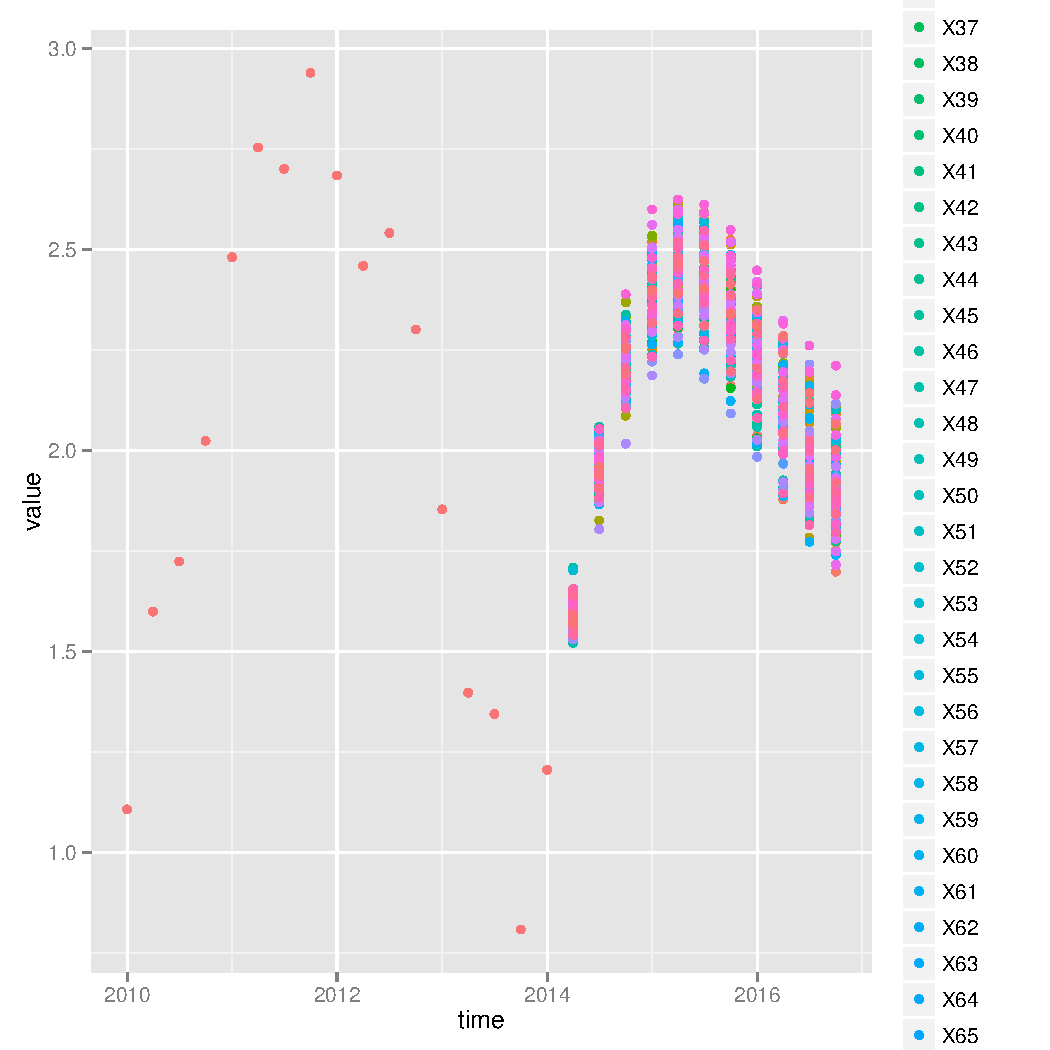
\includegraphics[width=\maxwidth]{figure/unnamed-chunk-7-1} 

\end{knitrout}




\end{document}
